\chapter{NEOS}
This chapter compares the \ac{neos} approach to established methods by evaluating upper cross-section limits on the boosted \ac{vbf} $HH\rightarrow4b$ analysis. This section is not intended to find the most stringent cross-section limits but rather to provide a fair comparison and present the potential \ac{neos} holds compared to more conservative methods.

Specifically, \ac{neos} is compared against cross-section upper limits retrieved with a maximum likelihood fit as explained in chapter \ref{sec:statistics} to the Higgs pair invariant mass $m_{HH}$ and a classifier \ac{nn} trained solely on separation for signal to background with a \ac{bce} loss function as of equation \ref{eq:bce}. Models are trained with the \ac{tomatos} \ac{nn} training framework developed for this purpose \citep{tomatos}, described in section \ref{sec:neos_training}. Both the training for \ac{neos} as well as the classifier use the same \ac{nn} architecture described in \ref{sec:event_classification}.

Figure \ref{fig:training_metrics} presents the result of the training for both the \ac{bce}-trained \ac{nn} and the neos \ac{nn}. While the loss function for the classifier converges for the validation dataset at about epoch 400 the cls \red{check 1e4 training}. Furthermore the Asimov significance of equation \ref{eq:asimov-significance}, typically used as a proxy for the statistical test at various optimization steps, shows no clear correlation to the \ac{bce}-trained \ac{nn} whereas the significance anti-correlates with the \ac{neos} loss function.


% As indicated in the sum, these counts can be spread across different bins in the case where your data is a histogram, but the formula is more commonly reduced to the 1-bin scenario that just deals with the overall numbers of signal and background events. In this case, we can then Taylor expand the logarithm to get

% $$Z_A = \sqrt{2((s+b)(s/b + \mathcal{O}(s/b) - s)} \approx s/\sqrt{b}~~~\mathrm{for}~s<<b.$$

show mit giffer, das up down sehr hin und her springt --> training mit guten cut 

\begin{figure}
    \centering
    \subfigure[]{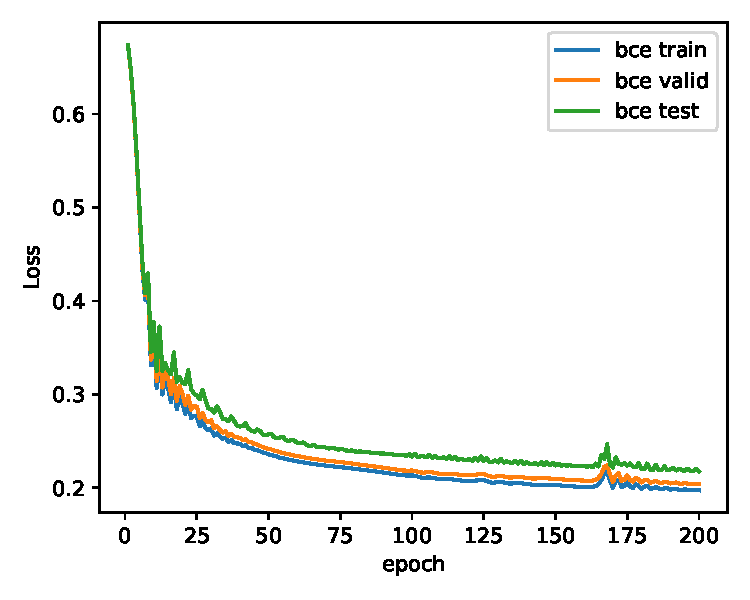
\includegraphics[width=.47\textwidth]{tomatos_bce_5_1000/bce.pdf}}
    \subfigure[]{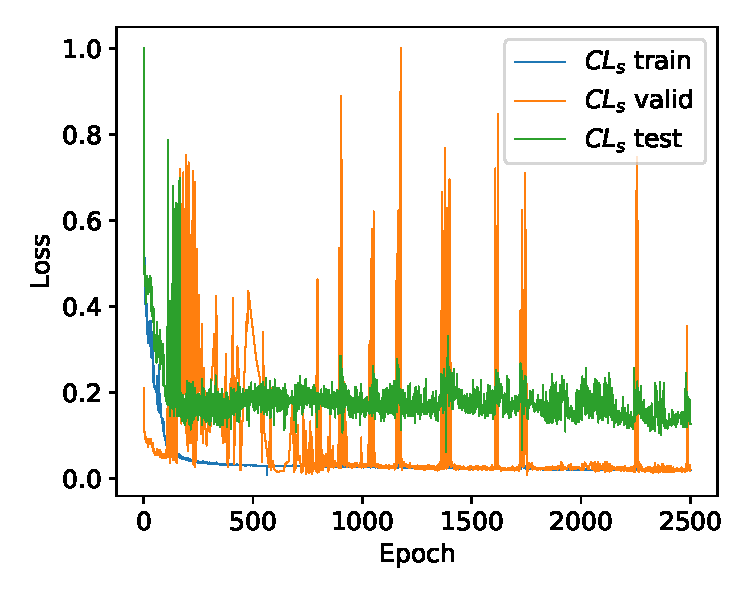
\includegraphics[width=.47\textwidth]{tomatos_cls_5_1000_unbound_shapesys/cls.pdf}} \\
    \subfigure[]{\includegraphics[width=.47\textwidth]{tomatos_bce_5_1000/hist.pdf}}
    \subfigure[]{\includegraphics[width=.47\textwidth]{tomatos_cls_5_1000_unbound_shapesys/hist.pdf}} \\
    \subfigure[]{\includegraphics[width=.47\textwidth]{tomatos_bce_5_1000/Z_A.pdf}}
    \subfigure[]{\includegraphics[width=.47\textwidth]{tomatos_cls_5_1000_unbound_shapesys/Z_A.pdf}} \\
    \caption[]{Loss function value for training, validation and test dataset per training epoch, resulting histograms for samples used in training and Asimov significance from top to bottom. \textbf{(Left column)} \ac{nn} trained with a \ac{bce} loss function. \textbf{(Right coloumn)} \ac{nn} trained with \ac{neos}. \red{redo all plots, significance wrong, make sure sys are same} }
    \label{fig:training_metrics}
\end{figure}


% \begin{figure}
%     \centering
%     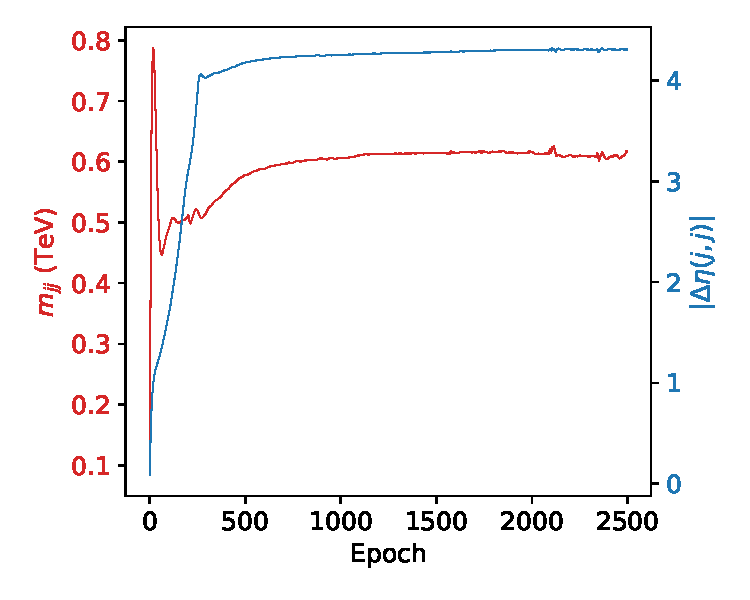
\includegraphics[width=1\textwidth]{tomatos_cls_5/cuts.pdf    }
%     \caption[]{Training metrics}
%     \label{fig:training_metrics}
% \end{figure}


After training these networks they are used in the analysis chain without the use of any \ac{neos} methods to determine limits on the cross-section with the \textit{cabinetry} fitting framework \citep{cranmer_2021_4627038}.

Each fit uses the same set of uncertainties determined from the highest ranked uncertainties of an $m_{HH}$ fit that used the full set of uncertainties shown in figure \ref{fig:m_hh_full_sys_ranking}.


\begin{figure}
    \centering
    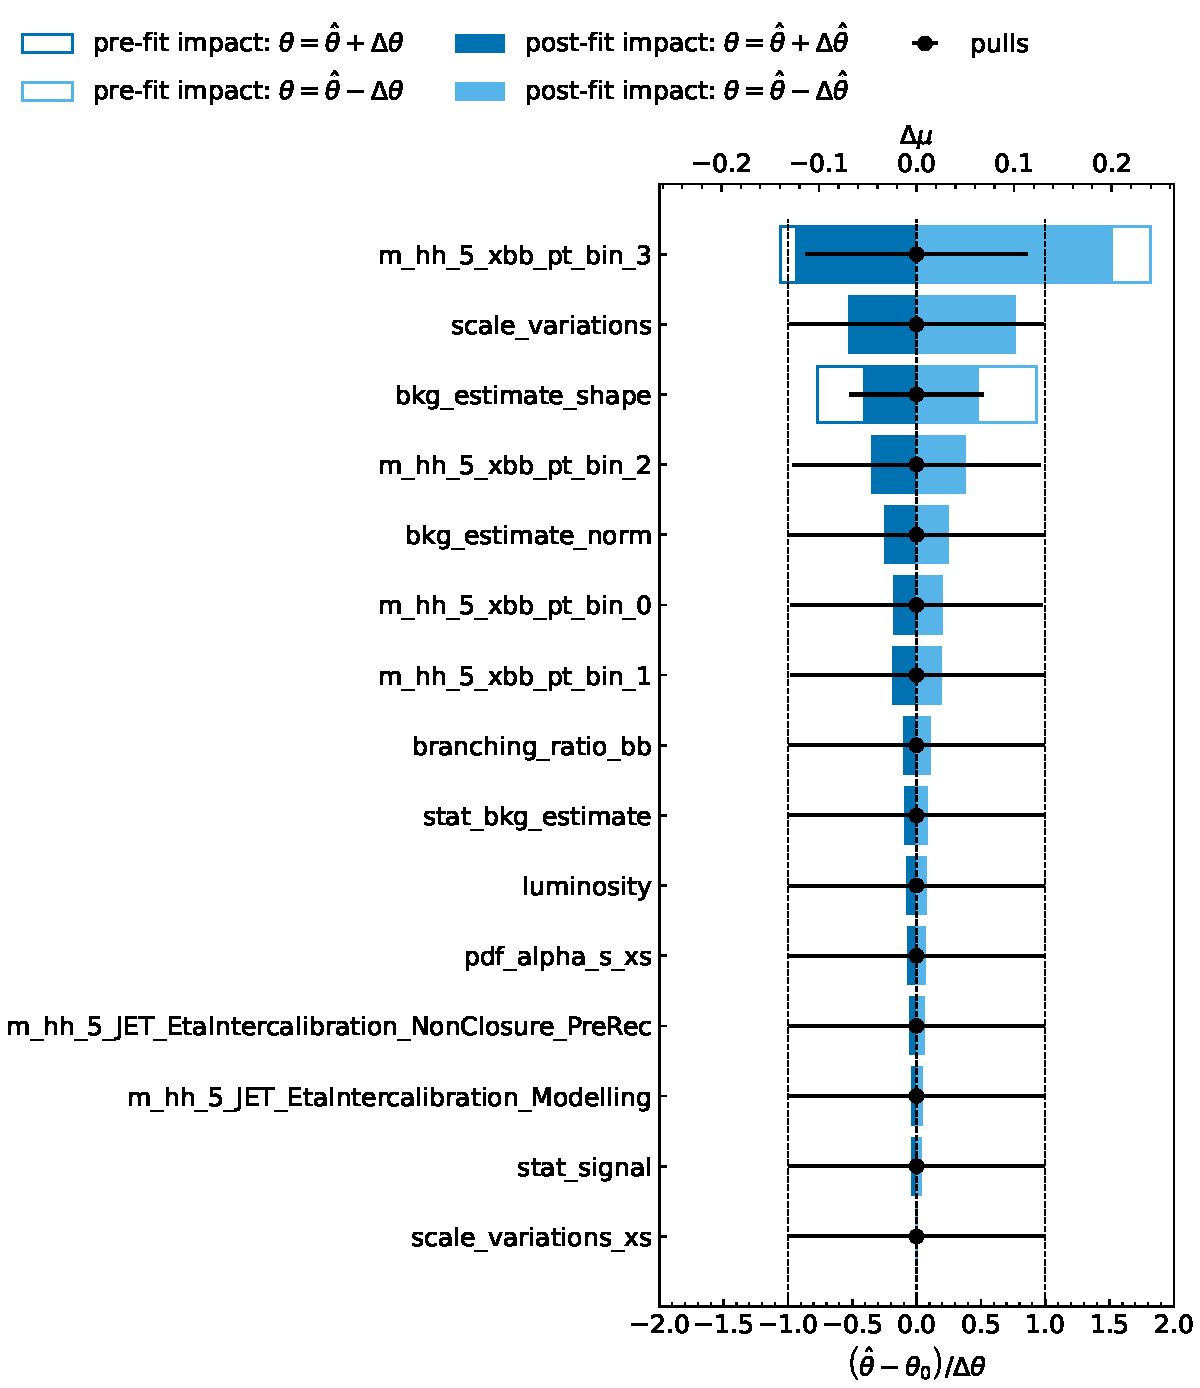
\includegraphics[width=1\textwidth]{m_hh_5_full_sys_ranking}
    \caption[]{\red{redo, not all uncertainties, but to illustrate}
        Nuisance parameter impact ranking ordered by their post-fit impact on the signal strength $\Delta\mu$ on the upper axis for an invariant Higgs Pair mass fit \mhh{}. The impact of a nuisance parameter $\Theta$ is assessed by performing four fits. In each fit, a nuisance parameter is fixed to its nominal best fit value $\hat{\Theta}$ plus a given nuisance parameter uncertainty $\Delta\Theta$ and computes the difference of the resulting $\mu_\text{fit}$ from this fit with the nominal best fitted value $\Delta\mu=\hat{\mu} - \mu_\text{fit}$. This is repeated for pre-fit $\pm\Delta\Theta$ and post-fit $\pm\Delta\hat{\Theta}$ uncertainties of $\Theta$. The lower axis and the black points represent the pull for each nuisance paramter, calculated as the difference between the best-fit value and the nominal pre-fit $(\hat{\Theta} - \Theta_0)$, divided by its variance $\Delta\Theta$ for the parameter $\Theta$. If the model is accurate, the expected value of each pull should be zero, with a variance of one, given a sufficiently large sample size. In this asymptotic limit the test statistic is computed from the sum of pulls and follows a $\chi^2$ distribution if the model is correct. Thus, pulls serve as goodness-of-fit quantities. }
    \label{fig:m_hh_full_sys_ranking}
\end{figure}

\red{also show gif training development?}


beide trainings metriken zeigen
alle fits mit allen plots + ranking
systematics vom ranking auch schon besprochen, hier auch nochmal kurz erwähnen

limit overlay

the improvement is blah


% \section{Performance Validation}

